\section{Experimentación}

\subsection{PageRank}
\subsubsection{Complejidad}

\begin{figure}[h]
\centering
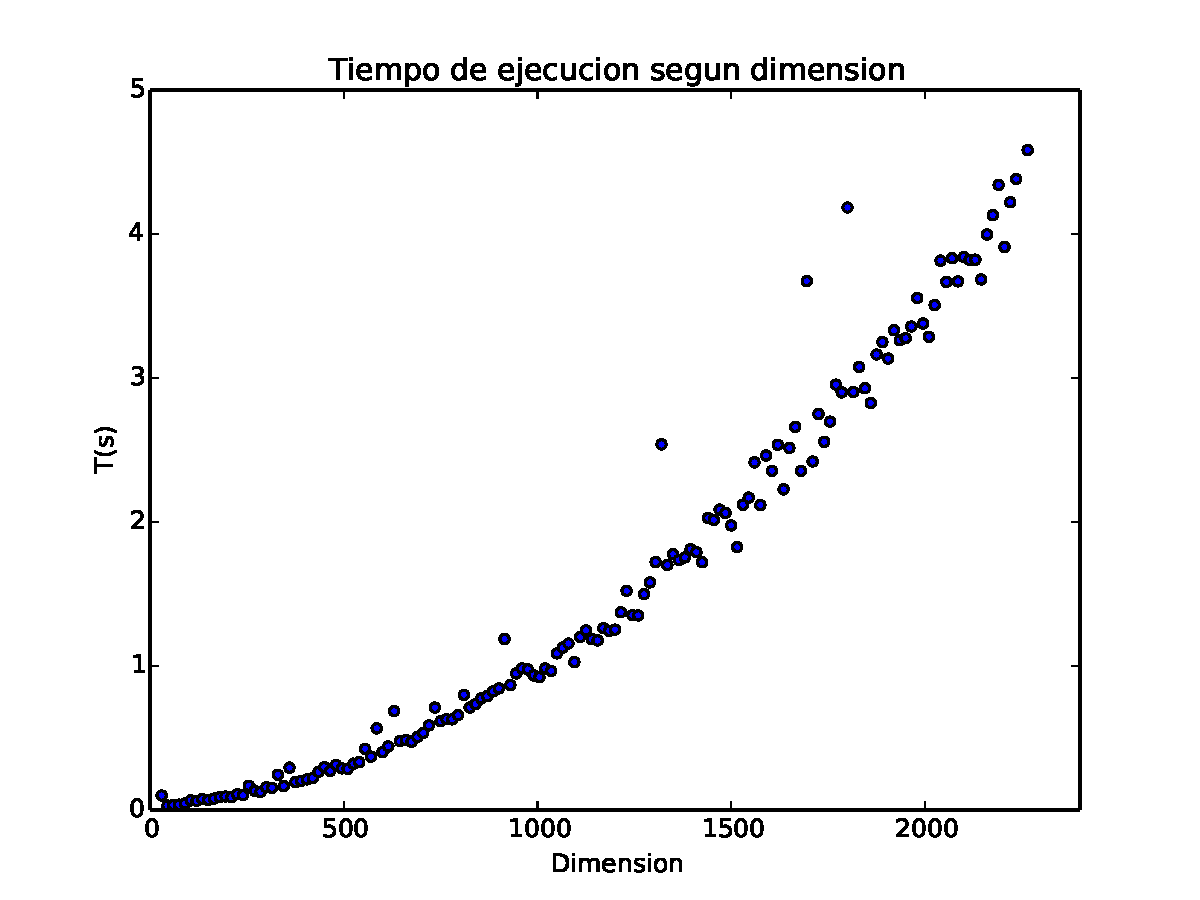
\includegraphics[scale=0.7]{images/complejidad.pdf}
\caption{Tiempos de ejecución según cantidad de webs.}
\label{timePageRank}
\end{figure}

\subsubsection{Casos Patologicos}
Caso particular chiquito, pagina 3. Fijate el parrafo que arranca en A simple apprroach...... y despues This approach ignores that... La idea es armar el mismo grafo y mostrar el mismo ejemplo jaja

\begin{figure}[h]
\centering
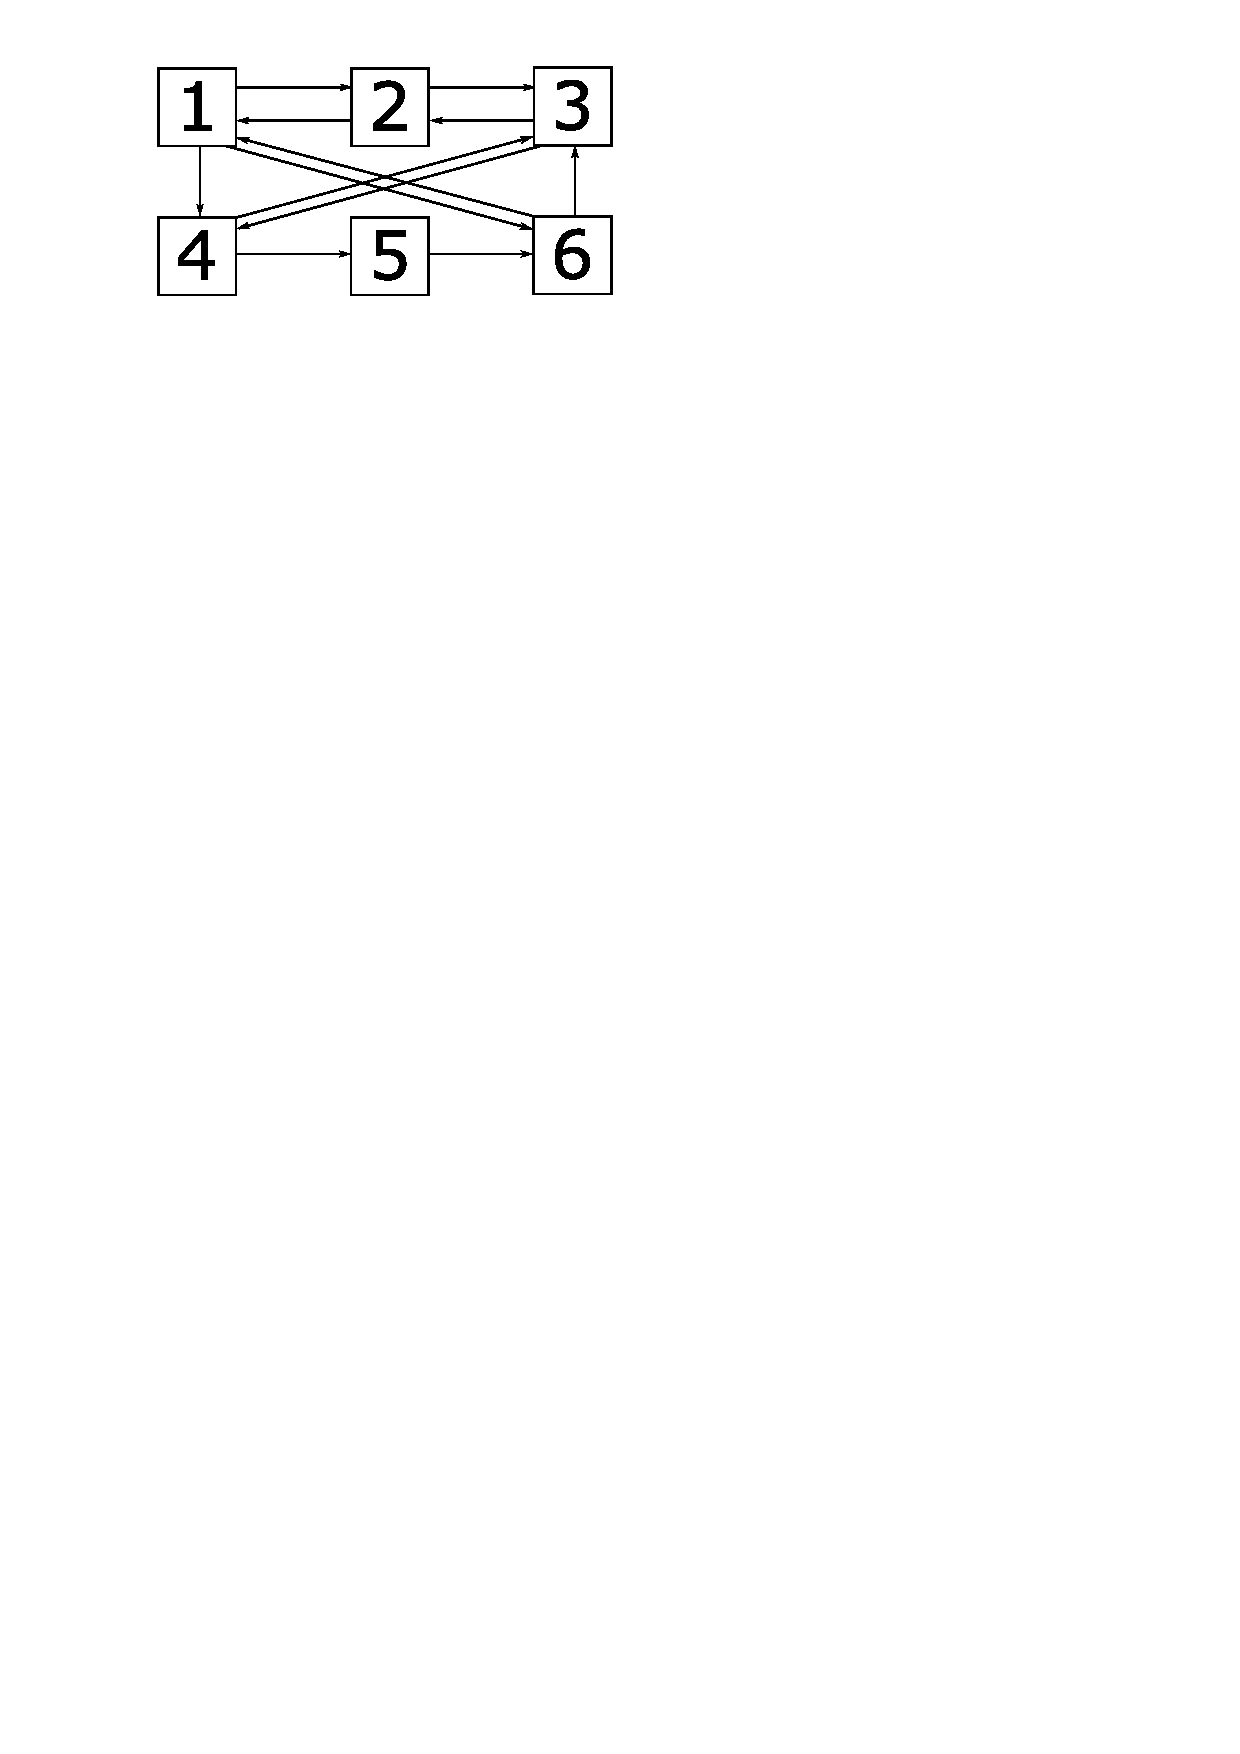
\includegraphics[scale=0.7]{images/drawing.pdf}
\caption{Caso de estudio}
\label{casoEst}
\end{figure}

\begin{table}[]
\centering
\caption{My caption}
\label{my-label}
\begin{tabular}{lll}
\hline
Nro. Web & PageRank & Por grado \\ \hline
1        & 0.164204 & 3         \\
2        & 0.172456 & 2         \\
3        & 0.237500 & 2         \\
4        & 0.172456 & 2         \\
5        & 0.098296 & 1         \\
6        &          & 2         \\ \hline
\end{tabular}
\end{table}

\subsection{Paginas Web}

\subsubsection{Comparacion PageRank vs In-Deg (RODRI)}
Comparar solo los rankings, nada de complejidad. Podes mencionar que In-Deg usa un algoritmo \order{n \times log(n)}, pero nada mas. Comparar top 10 con los dos y discutir diferenciias.

\subsubsection{Manipulacion}
Pagina 5, ejercicio 1. La idea es que plantees un caso de un tipo que quiere manipular el ranking, mostra que aunque agregues miles de nuevas paginas apuntando no podes hacer demasiado, hacelo en funcion de la cantidad de paginas que agregas?

Se puede manipular entonces o no? Agarra, en el eje x pone cantidad de sitios web que apuntan solamente al sitio u que le quiero subir el ranking, y en el eje y el ranking de ese sitio. Fijate que aumenta, y fijate si podes hacer algun tipo de curva de nivel con c (cuanto mayor c, mas manipulable es la cosa). Citar el paper de Sergei y Brin, que dicen que hacen promedios de muchas cosas en la practica para evitar este problema. Usan muchos criterios promediados.

\subsection{Ranking ATP}

Empezemos con el apartado que seguro el lector más esperaba de todo el t.p..Vilas fue o no 1ro entre 1975 y 1977? Esta pregunta podemos contestarla. Pero previo a esto, necesitamos poner al lector al tanto de la situación. Empecemos viendo los rankings oficiales de la época.


En 1975, Vilas llegó a la primera final de un Grand Slam, el Roland Garros, en donde fue derrotado por el sueco Björn Borg
y cuartos de final de Wimbledon.


Este es el top 10 para 1975 segun la ATP, donde Guillermo Vilas se hubica 2do:

\begin{eqnarray*}
173 & Jimmy & Connors \\
127 & Guillermo & Vilas \\
34 & Bjorn & Borg \\
19 & Arthur & Ashe \\
225 & Manuel & Orantes \\
210 & Ken & Rosewall \\
144 & Ilie & Nastase \\
180 & John & Alexander \\
318 & Roscoe & Tanner \\
309 & Rod & Laver 
\end{eqnarray*}

En 1976 la ATP hubica a Vilas 6to dentro del top 10:

\begin{eqnarray*}
173 & Jimmy & Connors \\
34 & Bjorn & Borg \\
144 & Ilie & Nastase \\
225 & Manuel & Orantes \\
288 & Raul & Ramirez \\
127 & Guillermo & Vilas \\
1 & Adriano & Panatta \\
134 & Harold & Solomon \\
87 & Eddie & Dibbs \\
41 & Brian & Gottfried 
\end{eqnarray*}

En 1977 Vilas se ubica segundo, por debajo de Connors. Recordemos que esto hasta el día de hoy sigue creando polémicas debido a los muy buenos resultados obtenidos por Vilas en aquel año comparados con los del estadounidense y que luego comentaremos.
Veamos el top 10 oficial para este año:

\begin{eqnarray*}
173 & Jimmy & Connors \\
127 & Guillermo & Vilas \\
34 & Bjorn & Borg \\
371 & Vitas & Gerulaitis \\
41 & Brian & Gottfried \\
87 & Eddie & Dibbs \\
225 & Manuel & Orantes \\
288 & Raul & Ramirez \\
144 & Ilie & Nastase \\
81 & Dick & Stockton 
\end{eqnarray*}

Todos los años tienen como lider indiscutido al estadounidense Jimmy Connors.

\subsubsection{Ranking ATP oficial vs. Ranking PageRank vs. Sort por diferencia de victorias/derrotas}

Introducimos aquí un algoritmo de rankeo con un criterio de ordenamiento basado en victorias/derrotas, que además, si hay empate define por diferencia de puntos, aunque para el caso de tenis y por como esta definido el sistema de puntos del mismo no tiene ninguna relevancia. Solo nos servirá para poder hacer un análisis cualitativo de las virtudes de pagerank sobre algoritmos más básicos y comparar estos resultados con el ranking oficial y poder obtener así alguna conclusión sobre los mótivos principales de la investigación.

Veamos que obtuvimos en cada año con este algoritmo, empezando por 1975:

\begin{eqnarray*}
id & PG & PP \\
19 & 96 & 18 \\
225 & 90  & 20 \\
127 & 86 & 18 \\
173 & 79 & 11 \\
144 & 88 & 22 \\
34 & 82 & 17 \\
288 & 70 & 28 \\
180 & 65 & 23 \\
318 & 64 & 24 \\
155 & 60 & 21 \\
\end{eqnarray*}

Podemos ver que Vilas no aparece segundo, si no tercero. Connors fue desplazado al 4to lugar y en primer lugar aparece Arthur Ashe quien ocupaba el lugar que Connors ocupa ahora. Podemos ver varios cambios relacionados al top 10 oficial. 

Todos ellos particularmente relacionados al hecho de que como se habia anticipado la cantidad de victorias sobre derrotas conformaria otro ranking diferente en el cual no importa exactamente que clase de victorias a conseguido o derrotas sufrido un determinado participante. Podemos ver que Vilas con más victorias sobre derrotas que Connors, se encontraba por debajo de él en el ranking oficial. Esto se debe al sistema de puntos manejados por el ATP donde se suma más puntaje cuanto mas avancemos en un torneo y cuantas más finales ganemos y por la jerarquía de ese torneo. Claramente no alcanza con ganar un solo torneo importante. Debemos tener continuidad y participación.

Observemos el ranking de 1976:

\begin{eqnarray*}
id & PG & PP \\
173 & 86 & 9 \\
127 & 83 & 20 \\
144 & 73 & 15 \\
288 & 91 & 33 \\
225 & 76 & 19 \\
87 & 83 & 28 \\
34 & 57 & 12 \\
318 & 71 & 27 \\
380 & 75 & 32 \\
134 & 70 & 27 \\
\end{eqnarray*}

Vemos que Vilas avanzó del 6to lugar al 2do puesto que era ocupado por  Bjorn Borg y que fue desplazado al 7mo. 

Si analizamos un poco los partidos veremos que Vilas fué derrotado por Bjorn Borg 3 veces (Winbledon, Dallas WCT, Sao Paulo WCT) mientras que Vilas nunca pudo derrotarlo. Contra Connors se enfrentó una vez y fue derrotado (US Open) al igual que Bjorn Borg, que se enfrentó en 3 ocaciones contra Connors y cayó en la misma cantidad...esto nuevamente es un indicador de que determinadas victorias son más importantes que otras.

Veamos que sucede en 1977:

\begin{eqnarray*}
id & PG & PP \\
127 & 126 & 14 \\
41 & 105 & 22 \\
34 & 71 & 8 \\
173 & 69 & 15 \\
87 & 77 & 28 \\
371 & 60 & 15 \\
225 & 65 & 25 \\
134 & 64 & 27 \\
288 & 61 & 24 \\
380 & 66 & 30 \\
\end{eqnarray*}

Ok. Tomemoslo con calma. Vilas aparece primero..pero esto no es indicador absoluto de que la ATP cometió un error debido a la falta de información que provee. Aunque si nos da indicios de lo que realmente pasó.

La diferencia de partidos ganados sobre perdidos con respecto a cualquier otro competidor es bastante significativa. Podemos ver que Connors fué desplazado al 4to lugar. Segundo se ubica Brian Gottfried, que durante ese año tuvo un gran desempeño, entre los que se encuentra su victoria sobre Vilas en la final del Roland Garros. 

Todos estos datos nos permiten dar una idea de hacia donde vamos..las posiciones parecen estar relacionadas con el desempeño del competidor durante ese año, es decir, cuantas finales disputó o que tan lejos avanzó en un torneo y a que rivales venció.

A priori..cantidad de victorias está relacionado con cantidad de puntos..pero esto no es una regla general y depende como mencionamos del sistema de puntajes. Para poder asemejar a la relevancia que la ATP le da a los torneos tenemos que utilizar un algoritmo que aproveche esa carácteristica lo mejor posible. Para esto haremos uso del modelo GeM y analizaremos sus resultados. Esperariamos que los mismos se parezcan al ranking oficial con ciertas variaciones, pero como minimo se mantengan los mismos en el top 10 que el ranking oficial. 

Utilizaremos los siguientes parámetros para generar los 3 rankings:

$c$ = 0.85
$\delta$ = 0.00001

Además, como indicamos en el diseño del sistema, usaremos una matriz de personalización uniforme, dado que no nos interesa que influyan sobre los resultados ninguna información estadistica de un torneo anterior, por el simple hecho de que evaluamos a los jugadores desde cero cada año.

Avancemos sobre los resultados, comenzando con 1975:

\begin{eqnarray*}
id & puntaje \\
19 & 0.033172 \\
34 & 0.030089 \\
225 & 0.026483 \\
144 & 0.026254 \\
127 & 0.023572 \\
173 & 0.021918 \\
180 & 0.017379 \\
318 & 0.015914 \\
309 & 0.011614 \\
210 & 0.011055 \\
\end{eqnarray*}

Vemos que Vilas se ubica en el 4to puesto, Connors fué desplazado al 5to puesto y por arriba se ubican Ashe en primer puesto y Borg en segundo lugar. 

Si analizamos los partidos vemos que Ashe se enfrentó en una sola oportunidad a Connors y logró derrotarlo, en lo que fué la final Wimbledon. Además se enfrento en 7 oportunidades a Borg y logró vencerlo en 4 (Wimbledon, Barcelona WCT, Dallas WCT, Munich WCT), siendo Wimbledon el más importante de los 7 enfrentamientos.

Borg obtuvo la final de Roland Garros frente a Vilas como máximo logro. 

Mientras tanto Manuel Orantes hizo lo propio para obtener el 3er lugar contra Vilas derrotandolo en las 4 oportunidades que se encontraron y derrotando a Connors en su único enfrentamiento. 
No es una tarea fácil determinar todas estas congruencias pero con un simple vistazo a los partidos jugados y los torneos en los que se enfrentaron parece claro que el ranking es elocuente.

Veamos el ranking de 1976:

\begin{eqnarray*}
id & puntaje \\
173 & 0.033300 \\
144 & 0.031773 \\
288 & 0.029343 \\
87 & 0.026328 \\
41 & 0.025002 \\
134 & 0.024189 \\
127 & 0.024006 \\
34 & 0.023806 \\
225 & 0.020587 \\
1 & 0.014804 \\
\end{eqnarray*}

No parace haber mucho que analizar con respecto al ranking oficial. Vilas se encuentra una posición mas abajo. Connors sigue siendo lider indiscutido y la otras posiciones relativas no han cambiado demasiado. Podriamos resaltar el caso particular de Borg que no tuvo malos resultados, destacando su final ganada contra Ilie Nastase en Wimbledon, una final perdida en el US Open contra Connors y Cuartos de final en un Roland Garros. Pero si miramos el mismo ranking pero por diferencia de ganados/perdidos veremos que Borg se encuentra casi en la misma posición debido a la poca cantidad de partidos ganados con respecto a los perdidos. 

Concluyamos con el análisis de 1977: 

\begin{eqnarray*}
id & puntaje \\
127 & 0.037046 \\
41 & 0.035463 \\
34 & 0.029461 \\
173 & 0.027319 \\
134 & 0.024189 \\
87 & 0.023230 \\
81 & 0.021816 \\
371 & 0.017483 \\
288 & 0.016667 \\
225 & 0.016318 \\
\end{eqnarray*}

Por una diferencia significativa, Vilas desplaza del primero puesto a Connors para quedarse el con el trono. Pero hay una razón bastante justificada para que esto suceda.
En 1977 Vilas conquistó 17 torneos (récord todavía vigente), se consagró en Roland Garros frente a Brian Gottfried por 6-0 6-3 6-0 y el US Open frente a Jimmy Connors por 2-6 6-3 7-6 6-0, fue finalista de Australia donde cayó frente a Roscoe Tanner por 3-6 3-6 3-6, logró una seguidilla de 50 partidos consecutivos sin conocer la derrota y, durante esos doce meses, ganó 145 de los 159 encuentros que jugó (91,1\%).
Jimmy Connors, en 1977 no obtuvo ningún torneo de Grand Slam y ganó ocho torneos, menos de la mitad de los logrados por Vilas. 
Parece lógico que Connors incluso este unos escalones más abajo en el ranking. Además el ranking por partidos ganados/perdidos para los primeros 4 es identico. Esto no puede hacer más que confirmar que Vilas fué primero indiscutido en 1977 por una amplia diferencia, sobre todo por el bajo rendimiento de Connors durante ese año. 

Como comentamos al principio, la cantidad de partidos ganados y los rivales derrotados son factores importantes a la hora de generar el ranking con un metodo como GeM. Las condiciones usadas son muy similares a la forma de rankeo que utiliza la ATP, por este motivo podemos concluir que el ranking de la ATP de 1977 con seguridad tiene un error de computo. Si la ATP hubiese cambiado a un sistema como el GeM pero con un sistema de puntos más especializado y las condiciones fueran retroactivas, hoy el número 1 indiscutido de 1977 sería sin lugar a dudas el gran willy.

\subsubsection{Eleccion del factor de 'teletransportacion' c (RODRI)}
probar relevancia a medida que cambias ese valor = 0.85, creo que c.

Citar paper de google, que usan 0.85. Discutir que si c es uno, ignoras la estructura del grafo al hacer el ranking, todos rankean igual.

Pagina 6.... This is the ultimately egalitarian case: the only... blah. La idea es jugar con c aca, como dije arriba. Es un buen exp, hay que pensar bien como graficarlo y que quede lindo, creo que es facil.

\subsection{Metodo de la Potencia}

\subsubsection{Representacion de la Matriz de Transicion (RODRI/FEDE)}
Este experimento lo pueden hacer directo o usando al PageRank. Si pueden, implementen todas las representaciones de matrices y luego comparen el tiempo de computo del producto N veces. Comparen la matriz normal vs el resto. Discutan que en paginas web la cantidad de vertices del grafo se va al carajo, pero para deportes es super acotada, asi que la eleccion de estructura no afecta tanto.

Aca podes argumentar que lo que domina al metodo de la potencia es la cantidad de productos, asi que no hace falta probar PageRank directo. Igual si queres metelo con pagerank de una, a fin de cuentas es lo mismo.

\subsubsection{Evolucion de la norma entre iteraciones}
Como va evolucionando la norma manhattan entre dos iteraciones sucesivas. Eje x, iteraciones, eje y, norma manhattan.

\subsubsection{Convergencia}
Aca tienen que calcular el vector posta, y luego tomar algun tipo de norma. En el eje x van a tener la cantidad de iteraciones, y en el eje y van a tener la norma de x* - $x_actual$.

\subsubsection{Eleccion del $x_0$}

Aca pongan que te conviene arrancar con una buena 'adivinanza' de la solucion, asi se acerca mas rapido. Muestren la cantidad de iteraciones a la convergencia (norma manhattan < epsilon) dependiendo de la distanciia de la solucion inicial a la solucion posta. Si arranco con la posta de una, converge de una. Si arranco con una sol asquerosa inicial, tarda mas iteraciones en cumplir nuestro epsilon.

Mostrar dos instancias, una donde arrarnco desde el valor inicial donde todos tienen 1/n y otra donde una tiene 1 y el resto 0, mostrar la cantidad de pasos y como evoluciona la norma.


